\onecolumn
\section*{A}
\label{sec:appendix}
\renewcommand{\theequation}{\thesection .\arabic{equation}}

\subsection*{Derivation of Gaussian elimination algorithm terms}
\label{sec:derivgauss}
Considering our generalised matrix
  \[A =
    \mqty[b_1 & c_1 & 0 & \hdots & \hdots & 0 \\
          a_1 & b_2 & c_2 & 0 & \hdots & 0 \\
          0 & a_2 & b_3 & c_3 & \hdots & 0 \\
          \vdots & \ddots & \ddots & \ddots & \ddots & \vdots \\
          0 & \hdots & \ddots & a_{n-2} & b_{n-1} & c_{n-1} \\
          0 & \hdots & \hdots & 0 & a_{n-1} & b_n],
  \]
we will obtain our algorithm from row reduction by subtracting the first row
times $\frac{a_1}{b_1}$ from the second row ($\text{I} - \frac{a_1}{b_1}\text{II}
$), and we see that the new diagonal element is given by
  \[\widetilde{b_2} \equiv b_2 - \frac{a_1}{b_1}c_1.\]
Considering eq. \ref{eq:matrixeq} then, the corresponding change on the left
hand side is given by
  \[\widetilde{d_2} \equiv d_2 - \frac{a_1}{b_1}d_1.\]
Performing the same operation on the next row
($\text{III} - \frac{a_2}{\widetilde{b_2}}\text{II}$), we get
  \[\widetilde{b_3} \equiv b_3 - \frac{a_2}{\widetilde{b_2}}c_2, \quad
  \widetilde{d_3} \equiv d_3 - \frac{a_2}{\widetilde{b_2}}\widetilde{d_2}.
  \]
Letting $\widetilde{b_1} \equiv b_1$, $\widetilde{d_1} \equiv d_1$, and
generalising, we get:
  \begin{equation}
    \widetilde{b_i} = b_i - \frac{a_{i-1}}{\widetilde{b}_{i-1}}c_{i-1}, \quad
    \widetilde{d_i} = d_i - \frac{a_{i-1}}{\widetilde{b}_{i-1}}\widetilde{d_{i-1}}.
  \end{equation}
  
\subsection*{Additional plots}

\begin{figure}[htbp]
	\centering
	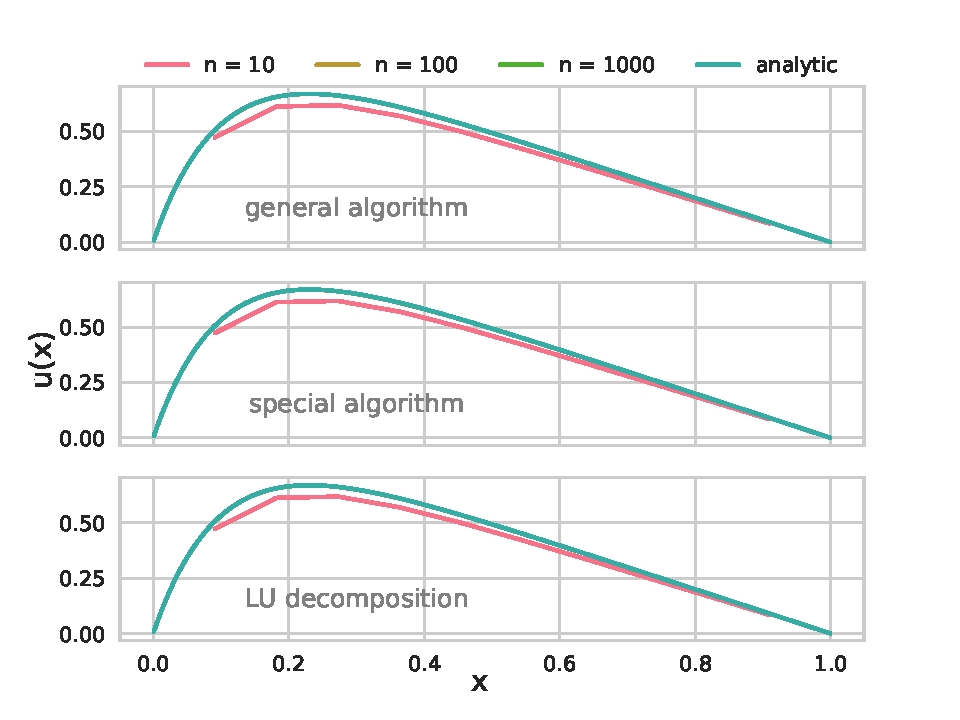
\includegraphics[width=\textwidth]{all_matrix_compare.pdf}
	\caption{The numeric solution using different solving algorithms. The graphs for n=100 and n=1000 are so similar that they are not distinguishable.}
	\label{fig:all}
\end{figure}